% Author: Dr. Matthias Jung, DL9MJ
% Year: 2021
\documentclass[convert = false, border=5pt]{standalone}
\usepackage{fontspec}
\setmainfont{Roboto}
\usepackage[siunitx, straightvoltages]{circuitikzgit}
\usepackage{tikz}


\usetikzlibrary{calc, positioning}

\begin{document}
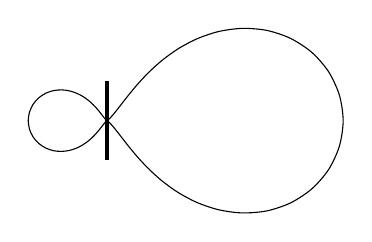
\begin{tikzpicture}
 \draw plot[
        variable=\t,
        domain=0:360,
        smooth,samples=51
    ] 
  ({50*sin(\t)}:{3*pow(sin(\t/2),5)});

 \draw plot[
        variable=\t,
        domain=0:360,
        smooth,samples=51
    ] 
  ({180+50*sin(\t)}:{1*pow(sin(\t/2),5)});

  \draw [very thick] (0,-0.5) -- (0,0.5);
\end{tikzpicture}
\end{document}
